\documentclass{standalone}
\usepackage{tikz, xcolor}
\usetikzlibrary{shapes,arrows}

\begin{document}

\begin{tikzpicture}[thick, scale=2.0]
\tikzstyle{vertexr}=[rectangle, draw=blue, thick, minimum size=14pt, inner sep=2pt]
\tikzstyle{vertexc}=[circle, draw=blue, thick, inner sep=2pt]
\tikzstyle{drawstyle}=[thick, ->]

\node[vertexr] (G0x0) at (0,0) {void Func cheyenne};
\node[vertexr] (G0x1) at (0,-1) {int a};
\node[vertexr] (G1x1) at (1,-1) {bool b};
\node[vertexr] (G2x1) at (2,-1) {char c};
\draw[drawstyle] (G1x1) -- (G2x1);
\draw[drawstyle] (G0x1) -- (G1x1);
\draw[drawstyle] (G0x0) -- (G0x1);
\node[vertexr] (G3x1) at (3,-1) {Compound};
\node[vertexc] (G3x2) at (3,-2) {.};
\draw[drawstyle] (G3x1) -- (G3x2);
\node[vertexr] (G4x2) at (4,-2) {Call output};
\node[vertexr] (G4x3) at (4,-3) {a};
\draw[drawstyle] (G4x2) -- (G4x3);
\node[vertexr] (G5x2) at (5,-2) {Call outputb};
\node[vertexr] (G5x3) at (5,-3) {b};
\draw[drawstyle] (G5x2) -- (G5x3);
\node[vertexr] (G6x2) at (6,-2) {Call outputc};
\node[vertexr] (G6x3) at (6,-3) {c};
\draw[drawstyle] (G6x2) -- (G6x3);
\node[vertexr] (G7x2) at (7,-2) {Call outnl};
\draw[drawstyle] (G6x2) -- (G7x2);
\draw[drawstyle] (G5x2) -- (G6x2);
\draw[drawstyle] (G4x2) -- (G5x2);
\draw[drawstyle] (G3x1) -- (G4x2);
\draw[drawstyle] (G0x0) -- (G3x1);
\node[vertexr] (G8x0) at (8,0) {void Func sioux};
\node[vertexr] (G8x1) at (8,-1) {int a};
\node[vertexr] (G9x1) at (9,-1) {bool b};
\node[vertexr] (G10x1) at (10,-1) {char c};
\draw[drawstyle] (G9x1) -- (G10x1);
\draw[drawstyle] (G8x1) -- (G9x1);
\draw[drawstyle] (G8x0) -- (G8x1);
\node[vertexr] (G11x1) at (11,-1) {Compound};
\node[vertexc] (G11x2) at (11,-2) {.};
\draw[drawstyle] (G11x1) -- (G11x2);
\node[vertexr] (G12x2) at (12,-2) {Call output};
\node[vertexr] (G12x3) at (12,-3) {a};
\node[vertexr] (G12x4) at (12,-4) {1};
\draw[drawstyle] (G12x3) -- (G12x4);
\draw[drawstyle] (G12x2) -- (G12x3);
\node[vertexr] (G13x2) at (13,-2) {Call outputb};
\node[vertexr] (G13x3) at (13,-3) {b};
\node[vertexr] (G13x4) at (13,-4) {2};
\draw[drawstyle] (G13x3) -- (G13x4);
\draw[drawstyle] (G13x2) -- (G13x3);
\node[vertexr] (G14x2) at (14,-2) {Call outputc};
\node[vertexr] (G14x3) at (14,-3) {c};
\node[vertexr] (G14x4) at (14,-4) {3};
\draw[drawstyle] (G14x3) -- (G14x4);
\draw[drawstyle] (G14x2) -- (G14x3);
\node[vertexr] (G15x2) at (15,-2) {Call outnl};
\draw[drawstyle] (G14x2) -- (G15x2);
\draw[drawstyle] (G13x2) -- (G14x2);
\draw[drawstyle] (G12x2) -- (G13x2);
\draw[drawstyle] (G11x1) -- (G12x2);
\draw[drawstyle] (G8x0) -- (G11x1);
\node[vertexr] (G16x0) at (16,0) {void Func comanche};
\node[vertexr] (G16x1) at (16,-1) {int z};
\draw[drawstyle] (G16x0) -- (G16x1);
\node[vertexr] (G17x1) at (17,-1) {Compound};
\node[vertexr] (G17x2) at (17,-2) {bool b};
\node[vertexr] (G18x2) at (18,-2) {char c};
\draw[drawstyle] (G17x2) -- (G18x2);
\draw[drawstyle] (G17x1) -- (G17x2);
\node[vertexr] (G19x2) at (19,-2) {=};
\node[vertexr] (G19x3) at (19,-3) {b};
\node[vertexr] (G19x4) at (19,-4) {2};
\draw[drawstyle] (G19x3) -- (G19x4);
\draw[drawstyle] (G19x2) -- (G19x3);
\node[vertexr] (G20x3) at (20,-3) {true};
\draw[drawstyle] (G19x2) -- (G20x3);
\node[vertexr] (G21x2) at (21,-2) {=};
\node[vertexr] (G21x3) at (21,-3) {c};
\node[vertexr] (G21x4) at (21,-4) {3};
\draw[drawstyle] (G21x3) -- (G21x4);
\draw[drawstyle] (G21x2) -- (G21x3);
\node[vertexr] (G22x3) at (22,-3) {'z'};
\draw[drawstyle] (G21x2) -- (G22x3);
\node[vertexr] (G23x2) at (23,-2) {Call sioux};
\node[vertexr] (G23x3) at (23,-3) {z};
\node[vertexr] (G24x3) at (24,-3) {b};
\node[vertexr] (G25x3) at (25,-3) {c};
\draw[drawstyle] (G24x3) -- (G25x3);
\draw[drawstyle] (G23x3) -- (G24x3);
\draw[drawstyle] (G23x2) -- (G23x3);
\draw[drawstyle] (G21x2) -- (G23x2);
\draw[drawstyle] (G19x2) -- (G21x2);
\draw[drawstyle] (G17x1) -- (G19x2);
\draw[drawstyle] (G16x0) -- (G17x1);
\node[vertexr] (G26x0) at (26,0) {int ga};
\node[vertexr] (G27x0) at (27,0) {bool gb};
\node[vertexr] (G28x0) at (28,0) {char gc};
\node[vertexr] (G29x0) at (29,0) {void Func main};
\node[vertexc] (G29x1) at (29,-1) {.};
\draw[drawstyle] (G29x0) -- (G29x1);
\node[vertexr] (G30x1) at (30,-1) {Compound};
\node[vertexr] (G30x2) at (30,-2) {int a};
\node[vertexr] (G31x2) at (31,-2) {bool b};
\node[vertexr] (G32x2) at (32,-2) {char c};
\draw[drawstyle] (G31x2) -- (G32x2);
\draw[drawstyle] (G30x2) -- (G31x2);
\draw[drawstyle] (G30x1) -- (G30x2);
\node[vertexr] (G33x2) at (33,-2) {=};
\node[vertexr] (G33x3) at (33,-3) {a};
\node[vertexr] (G33x4) at (33,-4) {1};
\draw[drawstyle] (G33x3) -- (G33x4);
\draw[drawstyle] (G33x2) -- (G33x3);
\node[vertexr] (G34x3) at (34,-3) {555};
\draw[drawstyle] (G33x2) -- (G34x3);
\node[vertexr] (G35x2) at (35,-2) {=};
\node[vertexr] (G35x3) at (35,-3) {b};
\node[vertexr] (G35x4) at (35,-4) {2};
\draw[drawstyle] (G35x3) -- (G35x4);
\draw[drawstyle] (G35x2) -- (G35x3);
\node[vertexr] (G36x3) at (36,-3) {true};
\draw[drawstyle] (G35x2) -- (G36x3);
\node[vertexr] (G37x2) at (37,-2) {=};
\node[vertexr] (G37x3) at (37,-3) {c};
\node[vertexr] (G37x4) at (37,-4) {3};
\draw[drawstyle] (G37x3) -- (G37x4);
\draw[drawstyle] (G37x2) -- (G37x3);
\node[vertexr] (G38x3) at (38,-3) {'z'};
\draw[drawstyle] (G37x2) -- (G38x3);
\node[vertexr] (G39x2) at (39,-2) {Call cheyenne};
\node[vertexr] (G39x3) at (39,-3) {666};
\node[vertexr] (G40x3) at (40,-3) {true};
\node[vertexr] (G41x3) at (41,-3) {'c'};
\draw[drawstyle] (G40x3) -- (G41x3);
\draw[drawstyle] (G39x3) -- (G40x3);
\draw[drawstyle] (G39x2) -- (G39x3);
\node[vertexr] (G42x2) at (42,-2) {Call cheyenne};
\node[vertexr] (G42x3) at (42,-3) {777};
\node[vertexr] (G43x3) at (43,-3) {false};
\node[vertexr] (G44x3) at (44,-3) {'d'};
\draw[drawstyle] (G43x3) -- (G44x3);
\draw[drawstyle] (G42x3) -- (G43x3);
\draw[drawstyle] (G42x2) -- (G42x3);
\node[vertexr] (G45x2) at (45,-2) {Call sioux};
\node[vertexr] (G45x3) at (45,-3) {a};
\node[vertexr] (G46x3) at (46,-3) {b};
\node[vertexr] (G47x3) at (47,-3) {c};
\draw[drawstyle] (G46x3) -- (G47x3);
\draw[drawstyle] (G45x3) -- (G46x3);
\draw[drawstyle] (G45x2) -- (G45x3);
\node[vertexr] (G48x2) at (48,-2) {Call comanche};
\node[vertexr] (G48x3) at (48,-3) {a};
\draw[drawstyle] (G48x2) -- (G48x3);
\node[vertexr] (G49x2) at (49,-2) {=};
\node[vertexr] (G49x3) at (49,-3) {ga};
\node[vertexr] (G49x4) at (49,-4) {1};
\draw[drawstyle] (G49x3) -- (G49x4);
\draw[drawstyle] (G49x2) -- (G49x3);
\node[vertexr] (G50x3) at (50,-3) {888};
\draw[drawstyle] (G49x2) -- (G50x3);
\node[vertexr] (G51x2) at (51,-2) {=};
\node[vertexr] (G51x3) at (51,-3) {gb};
\node[vertexr] (G51x4) at (51,-4) {2};
\draw[drawstyle] (G51x3) -- (G51x4);
\draw[drawstyle] (G51x2) -- (G51x3);
\node[vertexr] (G52x3) at (52,-3) {false};
\draw[drawstyle] (G51x2) -- (G52x3);
\node[vertexr] (G53x2) at (53,-2) {=};
\node[vertexr] (G53x3) at (53,-3) {gc};
\node[vertexr] (G53x4) at (53,-4) {3};
\draw[drawstyle] (G53x3) -- (G53x4);
\draw[drawstyle] (G53x2) -- (G53x3);
\node[vertexr] (G54x3) at (54,-3) {'g'};
\draw[drawstyle] (G53x2) -- (G54x3);
\node[vertexr] (G55x2) at (55,-2) {Call sioux};
\node[vertexr] (G55x3) at (55,-3) {ga};
\node[vertexr] (G56x3) at (56,-3) {gb};
\node[vertexr] (G57x3) at (57,-3) {gc};
\draw[drawstyle] (G56x3) -- (G57x3);
\draw[drawstyle] (G55x3) -- (G56x3);
\draw[drawstyle] (G55x2) -- (G55x3);
\node[vertexr] (G58x2) at (58,-2) {Call comanche};
\node[vertexr] (G58x3) at (58,-3) {ga};
\draw[drawstyle] (G58x2) -- (G58x3);
\node[vertexr] (G59x2) at (59,-2) {Compound};
\node[vertexr] (G59x3) at (59,-3) {int ga};
\node[vertexr] (G60x3) at (60,-3) {bool gb};
\node[vertexr] (G61x3) at (61,-3) {char gc};
\draw[drawstyle] (G60x3) -- (G61x3);
\draw[drawstyle] (G59x3) -- (G60x3);
\draw[drawstyle] (G59x2) -- (G59x3);
\node[vertexr] (G62x3) at (62,-3) {=};
\node[vertexr] (G62x4) at (62,-4) {ga};
\node[vertexr] (G62x5) at (62,-5) {1};
\draw[drawstyle] (G62x4) -- (G62x5);
\draw[drawstyle] (G62x3) -- (G62x4);
\node[vertexr] (G63x4) at (63,-4) {999};
\draw[drawstyle] (G62x3) -- (G63x4);
\node[vertexr] (G64x3) at (64,-3) {=};
\node[vertexr] (G64x4) at (64,-4) {gb};
\node[vertexr] (G64x5) at (64,-5) {2};
\draw[drawstyle] (G64x4) -- (G64x5);
\draw[drawstyle] (G64x3) -- (G64x4);
\node[vertexr] (G65x4) at (65,-4) {true};
\draw[drawstyle] (G64x3) -- (G65x4);
\node[vertexr] (G66x3) at (66,-3) {=};
\node[vertexr] (G66x4) at (66,-4) {gc};
\node[vertexr] (G66x5) at (66,-5) {3};
\draw[drawstyle] (G66x4) -- (G66x5);
\draw[drawstyle] (G66x3) -- (G66x4);
\node[vertexr] (G67x4) at (67,-4) {'s'};
\draw[drawstyle] (G66x3) -- (G67x4);
\node[vertexr] (G68x3) at (68,-3) {Call sioux};
\node[vertexr] (G68x4) at (68,-4) {ga};
\node[vertexr] (G69x4) at (69,-4) {gb};
\node[vertexr] (G70x4) at (70,-4) {gc};
\draw[drawstyle] (G69x4) -- (G70x4);
\draw[drawstyle] (G68x4) -- (G69x4);
\draw[drawstyle] (G68x3) -- (G68x4);
\node[vertexr] (G71x3) at (71,-3) {Call comanche};
\node[vertexr] (G71x4) at (71,-4) {ga};
\draw[drawstyle] (G71x3) -- (G71x4);
\draw[drawstyle] (G68x3) -- (G71x3);
\draw[drawstyle] (G66x3) -- (G68x3);
\draw[drawstyle] (G64x3) -- (G66x3);
\draw[drawstyle] (G62x3) -- (G64x3);
\draw[drawstyle] (G59x2) -- (G62x3);
\draw[drawstyle] (G58x2) -- (G59x2);
\draw[drawstyle] (G55x2) -- (G58x2);
\draw[drawstyle] (G53x2) -- (G55x2);
\draw[drawstyle] (G51x2) -- (G53x2);
\draw[drawstyle] (G49x2) -- (G51x2);
\draw[drawstyle] (G48x2) -- (G49x2);
\draw[drawstyle] (G45x2) -- (G48x2);
\draw[drawstyle] (G42x2) -- (G45x2);
\draw[drawstyle] (G39x2) -- (G42x2);
\draw[drawstyle] (G37x2) -- (G39x2);
\draw[drawstyle] (G35x2) -- (G37x2);
\draw[drawstyle] (G33x2) -- (G35x2);
\draw[drawstyle] (G30x1) -- (G33x2);
\draw[drawstyle] (G29x0) -- (G30x1);
\draw[drawstyle] (G28x0) -- (G29x0);
\draw[drawstyle] (G27x0) -- (G28x0);
\draw[drawstyle] (G26x0) -- (G27x0);
\draw[drawstyle] (G16x0) -- (G26x0);
\draw[drawstyle] (G8x0) -- (G16x0);
\draw[drawstyle] (G0x0) -- (G8x0);
\end{tikzpicture}
\end{document}
Number of warnings: 0
Number of errors: 0
